\documentclass{IOS-Book-Article}     %[seceqn,secfloat,secthm]
\usepackage{mathptmx}
\usepackage{soul}\setuldepth{article}

%\normalfont
%\usepackage[T1]{fontenc}
%\usepackage{times}
%\usepackage[mtplusscr,mtbold]{mathtime}
\def\hb{\hbox to 11.5 cm{}}
%\usepackage[utf8]{inputenc}
%\usepackage[english]{babel}
\usepackage{graphicx}
\usepackage{textcomp}
%\usepackage{xcolor}
\usepackage{booktabs}
\usepackage{tabulary}
\usepackage{tabularx}
\usepackage{csquotes}
\usepackage{siunitx}
\usepackage[disable]{todonotes}
%\usepackage{natbib} % does not seem to work with ios 1
\newcommand{\citet}{\cite}% citet is not defined without natbib
\newcommand{\citep}{\cite}% citep is not defined without natbib
\setlength{\marginparwidth}{2.1cm}% enough space for todonotes
\usepackage{listings}
\usepackage{aurl}
\daurl{ob}{http://www.snik.eu/ontology/bb/}
\daurl{bb}{http://www.snik.eu/ontology/bb/}
\daurl{meta}{http://www.snik.eu/ontology/meta/}
\lstset{language=SPARQL,breaklines=true}
\usepackage[noabbrev,capitalize]{cleveref}
\newcommand{\snikversion}{1.3.0}
\newcommand{\snikversionlink}{\href{https://github.com/snikproject/ontology/releases/tag/\snikversion}{\snikversion}}
\newcommand{\sniktriples}{81499}
% SELECT (COUNT(DISTINCT *) AS ?count) {?s a owl:Class. FILTER(STRSTARTS(STR(?s),"http://www.snik.eu/ontology/"))}
\newcommand{\snikclasses}{4107}
% SELECT (COUNT(DISTINCT ?s) AS ?count) {{?s a rdf:Property.} UNION {?s a owl:ObjectProperty.} UNION {?s a owl:DataTypeProperty.} FILTER(STRSTARTS(STR(?s),"http://www.snik.eu/ontology/"))}
\newcommand{\snikproperties}{65}
%SELECT (COUNT(DISTINCT *) AS ?links) {?s ?p ?o. FILTER(STRSTARTS(STR(?o),"http://dbpedia")) }
\newcommand{\sniklinks}{579}

\begin{document}

\pagestyle{headings}
\def\thepage{}

\begin{frontmatter}              % The preamble begins here.


%\pretitle{Pretitle}
\title{SNIK: Textbook Knowledge on Hospital Information Management as Linked Data}
%\thanks{This work is supported by the DFG (German Research Foundation) under the Project SNIK, Grant no. 1605/7-1 and 1387/8-1.}%bug: will create an empty first page

\markboth{}{May 2022\hb}
%\subtitle{}

\author[A]{\fnms{Konrad} \snm{Höffner}%
%\thanks{Corresponding author: Konrad Höffner, Institute for Medical Informatics, Statistics and Epidemiology, Leipzig University,
\thanks{Corresponding author: Konrad Höffner, IMISE, Leipzig University,
Härtelstraße 16--18, 04107 Leipzig, Germany; E-mail: konrad.hoeffner@imise.uni-leipzig.de.}},
\author[A]{\fnms{Franziska} \snm{Jahn}},
\author[A]{\fnms{Birgit} \snm{Schneider}},
\author[A]{\fnms{Thomas} \snm{Pause}},
\author[A]{\fnms{Alfred} \snm{Winter}}
\runningauthor{K. Höffner et al.}
%\address[A]{Institute for Medical Informatics, Statistics and Epidemiology (IMISE), Leipzig University, Germany}
\address[A]{IMISE, Leipzig University, Germany}
%Medical Informatics, Management of Health Information Systemsi
%Härtelstraße 16--18, D-04107 Leipzig

\iffalse
\author{\IEEEauthorblockN{Konrad Höffner}
\IEEEauthorblockA{\textit{Institute for Medical Informatics, Statistics and Epidemiology} \\
\textit{Leipzig University}\\
Leipzig, Germany \\
\url{https://orcid.org/0000-0001-7358-3217}}
\and
\IEEEauthorblockN{Franziska Jahn}
\IEEEauthorblockA{\textit{Institute for Medical Informatics, Statistics and Epidemiology} \\
\textit{Leipzig University}\\
Leipzig, Germany \\
\url{https://orcid.org/0000-0002-7687-8544}}
\and
\and
\IEEEauthorblockN{Alfred Winter}
\IEEEauthorblockA{\textit{Institute for Medical Informatics, Statistics and Epidemiology} \\
\textit{Leipzig University}\\
Leipzig, Germany \\
%alfred.winter@imise.uni-leipzig.de}
\url{https://orcid.org/0000-0003-0179-954X}}
\and
\IEEEauthorblockN{Thomas Pause}
\IEEEauthorblockA{\textit{Institute for Medical Informatics, Statistics and Epidemiology} \\
\textit{Leipzig University}\\
Leipzig, Germany \\
\url{https://orcid.org/0000-0001-5832-4890}}
}
\fi
\begin{abstract}
%Textbooks contain abstract knowledge about a domain.
Textbooks about information management in hospitals describe the planning, monitoring and directing of a hospital's information system.
SNIK consists of the manually transformed content of three such textbooks as Linked Open Data.
The data model describes information management functions, roles executing these functions and the information used or updated by these functions.
%SNIK provides applications that are used to teach students internationally.
%and the result of applying the data model to three textbooks, an interview and a standard.
%To compare, 
%, making it a natural fit for RDF, RDFS and OWL.
%As the domain is large and highly relevant to students of Medical Informatics, modelling the knowledge is not only possible but also very useful.
We publish the result over several interfaces that are useful for researchers, administrators or students, depending on their objectives and capabilities.
\end{abstract}

% SWJ style
%\begin{keyword}
%\kwd{information management, information systems, hospital information management}
%\end{keyword}
% ICSCR style
%\begin{IEEEkeywords}
%linked open data, information management
%\end{IEEEkeywords}

% MIE style
\begin{keyword}
linked open data \sep information management
\end{keyword}
\end{frontmatter}

\section{Introduction}
A health information system (HIS) is the socio-technical subsystem of a care delivery organization~\citep{bb}.
This includes its different application systems, computers, and network components as well as their users.
A HIS processes data, information, and knowledge and its management involves planning, monitoring and directing those activities.
Due to the complexity and the unique conditions in health care, HIS management is an challenging task.
There are many different frameworks, textbooks and articles describing the scope of HIS management from the perspective of medical informatics.
%However, the disciplines of business informatics and information systems (IS) provide an even broader view on information systems and their management.
%A structured representation of the different perspectives leads to a holistic view on HIS management and helps help researchers and students connect their existing knowledge with further knowledge from other sources during research and learning.
In order to integrate different knowledge sources and to provide the knowledge in a structured, machine-readable data format, we extracted knowledge about HIS management from several sources, see \cref{tab:source}.
%three textbooks~\citep{bb,ob,he} and other sources, see \cref{tab:source}.
%\section{Sources}\label{sec:sources}
Three textbooks provide different views on the domain of Hospital Information Management:
\citet{bb} presents a broad view on \enquote{typical architectures of health information systems and their systematic strategic management}.
\citep{ob} concentrates on the \emph{tactical} management of information systems in general and on healthcare in particular.
The focus of tactical management lies on the planning and operation of projects.
\citet{he} explains information management beyond the scope of healthcare.
Other sources are interviews and standards.
%CIOX is based on an interview with the CIO of the Universitätsklinikum Leipzig.
%IT4IT is based on the IT4IT standard.\todo{Sebastian: Was über Standards und IT4IT schreiben}
%
The combination of this knowledge~\citep{semantischesnetz,domaene,approachtosupport} results in SNIK, the Semantic Network of Information Management in Hospitals (\enquote{Krankenhaus} in German).

In order to encourage and enable other researchers, students and health informatics professionals to use available knowledge of HIS management, we introduce different user interfaces to the SNIK ontology and discuss their suitability for different use cases of the target audiences.
%We discuss advantages and disadvantages of the interfaces and give recommendations on which ones present the best compromise for different use cases and target audiences.
%We conclude with plans for future work on interlinking and visualization.

%As the domain is large and highly relevant to students of Medical Informatics, modelling the knowledge is not only possible but also very useful.
Medical informatics students, who are trained for executive positions in information management departments of healthcare institutions, such as hospitals, need a clear terminology of their domain.
Due to different frameworks and textbooks dealing with information management in healthcare, modelling the knowledge unravels the links between the different views on information management.
These are only implicitly known or not known at all by experts in the field.
%
We present a common data model for the domain and the result of applying the data model to three textbooks.
We publish the result over several interfaces that are useful for researchers, practitioners and students, depending on their objectives and their Semantic Web skills.
%
Publishing textbook knowledge as Linked Data enables different ways of teaching.
%The data is continously revised: users constantly report wrong or missing data in the visualization, which is then corrected, respectively revised, by the researchers of the project.

\begin{table}[tbh]
\caption{The different ontologies and graphs of SNIK and their sources.
The namespace of each ontology is is equal to its URL with a slash suffix.
The graph group URL has no associated ontology and is the entry point of the RDF browser.
%All graphs are combined in the graph group \lowercase{\url{http://www.snik.eu/ontology}}.
}
\label{tab:source}
\begin{center}
%\begin{tabular}{\columnwidth}{lll}
\begin{tabular}{lll}
\toprule
\textbf{Prefix}	&\textbf{Ontology and Graph URL}			&\textbf{Source}\\		
\midrule
meta			&\url{http://www.snik.eu/ontology/meta}		&Meta Model\\
bb				&\url{http://www.snik.eu/ontology/bb}		&Textbook~\cite{bb}\\
ob				&\url{http://www.snik.eu/ontology/ob}		&Textbook~\cite{ob}\\
he				&\url{http://www.snik.eu/ontology/he}		&Textbook~\cite{he}\\
ciox			&\url{http://www.snik.eu/ontology/ciox}		&CIO Interview\\
it4it			&\url{http://www.snik.eu/ontology/it4it}	&Standard~\cite{it4it}\\
\midrule
sniko			&\url{http://www.snik.eu/ontology}			&Combined Graph Group\\
\bottomrule
\end{tabular}
\end{center}
\end{table}

\section{Methods}
\iffalse
\begin{figure}[h]
    \centering
    \includegraphics[width=0.5\columnwidth]{img/hierarchy.pdf}
    \caption{Excerpt of the SNIK class hierarchy. Source: \cite{snikposter}.}
	\label{fig:hierarchy}
\end{figure}
\fi
\vspace{-3pt}
In order to specify, which information should be extracted from the books and to facilitate comparisons, we use a common data model.
Because processed textbooks contain abstract knowledge instead of information about any specific hospital, all concepts are modelled as classes.
We thus call our data model the \enquote{meta model} in accordance with the term's definition as a shared modelling language~\citep[p.~8]{ob}.
The meta model (see \cref{fig:metamodel}) provides a common vocabulary for the domain of HIS management and thus defines, which superclasses and property can be used.
SNIK version \snikversionlink{} comprises five subontologies that are built upon the meta model, see Table 1.
%At the head of the class hierarchy (see \cref{fig:hierarchy}) is the \enquote{Top} class, which has exactly three disjunctive subclasses.
At the head of the class hierarchy is the \enquote{Top} class, which has exactly three disjunctive subclasses.
%
Following the meta model, each class has to be a subclass of exactly one of them.
The correct superclass of a new concept can be found by answering the question: Who (\enquote{Role}) does what (\enquote{Function}) and which information (\enquote{EntityType}) is needed? If a concept is neither of them, it cannot be modeled using the meta model.
As the subclass relation is transitive, a new class can be placed further down the hierarchy and it can still be inferred, whether it is a Function, Role or EntityType (see Figure 3).
Besides the subclass relationship, two classes can be connected with relations provided by the meta model.
The generic \enquote{is associated with} relationship carries little information.
For example, a role and a function can be connected as \enquote{is involved in} \enquote{is responsible for} and \enquote{approves}.
Relations that are neither of them can either be modeled by using the generic \enquote{is associated with} relation or by creating and using a new sub relation of \enquote{is associated with}
%
As a concession to practicality, we express each geleral rule extracted from a textbook as a single triple using classes as subject and object, and a property of the meta model.
For example, the rule "the CEO is involved in project reviews" is modelled as \enquote{\texttt{:Ceo} \aurl{meta}{isInvolvedIn} \texttt{:ProjectReview}.}, where \texttt{:Ceo} is a subclass of \aurl{meta}{Role} and \aurl{meta}{ProjectReview} is a subclass of \aurl{meta}{Function}.
While an OWL restrictions using \aurl{owl}{someValuesFrom} and \aurl{owl}{allValuesFrom} would be technically correct, the knowledge is not expressed that specifically in the textbooks.
Additionally, encoding each fact as a single triple facilitates tool support and prevents inconsistencies through non-atomic changes.

%\section{Data Quality}
%- extractors not always same people who wrote book/part of book
%- mistake when extracting
%- reasoning does not work (test)
%\begin{itemize}
%\item Multiple Subtops
%\item Inconsistent Subtop with Subclass
%\item SKOS Link to Different Subtop
%\item Subclass Cycles
%\item Missing superclass
%\item Undefined Objects
%\item Domain Violation
%\item Range Violation
%\item Class URL Naming Convention Violations
%\item Property URL Naming Convention Violations
%\item Missing Definition
%\item Literals with Semicolons
%\item Classes with too many subclasses
%\item No Restriction
%\item Non-HTTP URI
%\item OWL 2 DL: Undefined Properties
%\item OWL 2 DL: Multiply Defined Properties
%\item OWL 2 DL: Class Typing Constraints
%\end{itemize}
%-> use SHAPE/SHACL ?


\begin{table}
\caption{Access Options and Details.%
%KBox usage example: \texttt{pip install kbox \&\& kbox -kb http://www.snik.eu/ontology -install -server}.%doesn't work right now
}
\label{tab:access}
\begin{tabulary}{\columnwidth}{lL}
\toprule
URL						&\url{http://www.snik.eu/ontology}\\
Version					&\snikversionlink{}\\
%License					&CC BY-NC-SA 4.0\\
License					&Attribution-NonCommercial-ShareAlike 4.0 International (\href{https://creativecommons.org/licenses/by-nc-sa/4.0/}{CC BY-NC-SA 4.0})\\
Documentation	&\url{https://snikproject.github.io/ontology/}\\
SPARQL Endpoint			&\url{http://www.snik.eu/sparql}\\
LOD Cloud				&\url{https://lod-cloud.net/dataset/snik}\\
%Datahub				&\url{https://datahub.io/imise/snik/v/1}\\%offline
%Docker
KBox~\cite{kbox} Graph	&\url{http://www.snik.eu/ontology}\\
RDF Browser				&\url{http://www.snik.eu/ontology}\\
Visualization			&\url{http://www.snik.eu/graph}\\
Download				&\url{https://github.com/snikproject/ontology/archive/refs/tags/\snikversion.zip}\\
Figshare				&\url{https://doi.org/10.6084/m9.figshare.17057084.v1}\\
\bottomrule
\end{tabulary}%The source code for the services is available at \url{https://github.com/imise}
\end{table}

\iffalse
\begin{table}
\caption{Statistics}
\label{tab:statistics}
\centering
\begin{tabulary}{\columnwidth}{lS}
\toprule
\textbf{Category}					&\textbf{Count}\\
\midrule
Triples								&\sniktriples{}\\
Classes								&\snikclasses{}\\
Properties							&\snikproperties{}\\
Internal Links						&360\\
Links to HITO~\citep{hitometh2}  	&260\\
Links to DBpedia~\citep{dbpedia} 	&\sniklinks{}\\
%Subontologies	&\url{http://www.snik.eu/ontology/bb}\\
%		&\url{http://www.snik.eu/ontology/ciox,}\\
%		&\url{http://www.snik.eu/ontology/ob}\\
%		&\url{http://www.snik.eu/ontology/he}\\
%		&\url{http://www.snik.eu/ontology/it4it}\\
\bottomrule
\end{tabulary}%The source code for the services is available at \url{https://github.com/imise}
\end{table}
\fi

\begin{figure*}
\caption{The SNIK meta model}
\label{fig:metamodel}
\centering
%\includegraphics[width=0.9\textwidth]{img/metamodel9s.pdf}%7 page version
\includegraphics[width=0.7\textwidth]{img/metamodel9s.pdf}
\end{figure*}


%\section{Data Model}\label{sec:architecture}
%The initial structure of the meta model is defined in \citet{domaene}.
%The \enquote{meta model} defines three basic disjunctive classes and their possible relations: Roles (who), Function (does what) and Entity Types (and which information is therefore needed).
%A set of modular subontologies define subclasses of those three classes and their relations as described by a certain knowledge source about information management in hospitals:
%The \textbf{Semantic Network of Information Management in Hospitals} (SNIK\footnote{Hospital means \enquote{Krankenhaus} in German.}) is a modular OWL 2 DL ontology.
%from different sources:% three textbooks, an interview and a standard.


\iffalse
\section{Data Set Description}\label{sec:dsd}
\begin{table*}
\caption{use of established vocabularies}
\label{tab:templates}
\begin{tabulary}{\textwidth}{lL}
\toprule
\textbf{Vocabulary}	&\textbf{Description}\\
\midrule
&\\
&\\
&\\
\bottomrule
\end{tabulary}
\end{table*}
\fi

%\section{Data Transformation Process}
%\subsection{Interlinking}
%As shown in \cref{...}, we aligned our dataset to several others:
%We manually aligned our dataset to HITO, the Health IT Ontology~\citep{hitometh2}
%We automatically aligned our dataset to:
%- DBpedia~\citep{dbpedia}, as  
%- 
%\section{Lifecycle}\label{sec:application}
\section{Results}\label{sec:application}
\iffalse
\begin{figure}[ht]
\caption{The SNIK lifecycle}
\label{fig:lifecycle}
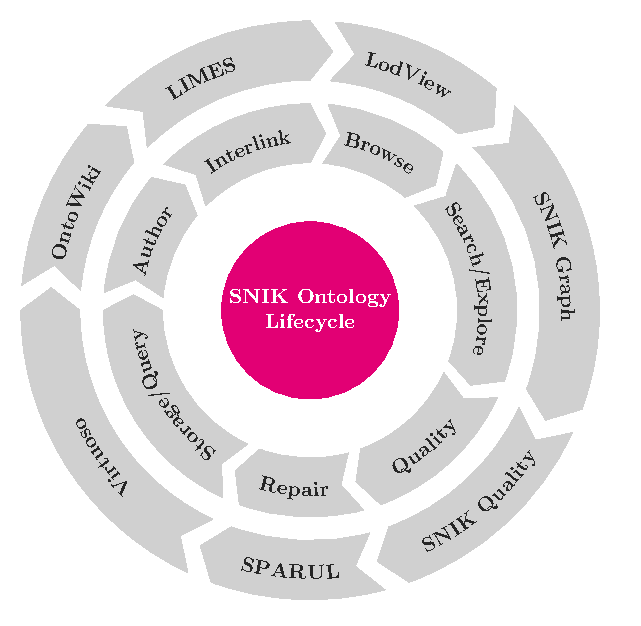
\includegraphics[width=0.5\columnwidth]{cycle.pdf}
\end{figure}
\fi
When we add a new textbook to SNIK, we identify all concepts that fit the meta model and their relations to other concepts.
Some project members are not proficient in RDF serializations, so we first fill out a meta model conforming spreadsheet template.
We then use Tarql\footnote{\url{https://github.com/cygri/tarql}} with a mapping configuration file\footnote{\url{https://github.com/snikproject/snik-csv2rdf}} to convert that spreadsheet to RDF.
Next, we refine the data in Protégé and upload it to a Virtuso SPARQL endpoint.
%After the initial publish phase, we describe the repeating steps of the reuse phrase with the SNIK lifecycle in \Cref{fig:lifecycle}:
\begin{enumerate}
\item the Virtuoso SPARQL endpoint is used for querying and as data source for all our applications  
\item an instance of the OntoWiki~\citep{ontowiki} is used for punctual changes and additions by non-Semantic-Web-experts, supplemented by SPARUL for changes involving large numbers of classes 
\item LIMES~\citep{limes} generates interlink candidates between the different textbooks, which can be approved or rejected by the users.
\aurl{skos}{closeMatch} is used instead of \aurl{owl}{equivalentClass} to emphasize that not only the names of concepts may differ between textbooks but there may be subtle differences in meaning as well.
We do not intent to express different treatment, such as reasoning, due to the theoretical difference between \aurl{skos}{Concept} and \aurl{owl}{Class}.
Links to HITO and DBpedia are created as well.%, see \cref{tab:statistics}.
\item LodView\footnote{\url{https://lodview.it/}} lets the user browse among the classes of SNIK and view particular classes in detail
\item SNIK Graph, detailed in \Cref{sec:snik-graph}, supplements the RDF browser by visualizing the relationships between classes.
Users often discover incorrect modelling or possibilities for enhancement in SNIK graph.
\item SNIK quality is a web application that uses SPARQL queries to find problems of varying degree, such as violations of domain, range or naming conventions, subclass cycles or missing definitions.
\item Problems suggested by users and SNIK quality are verified, solved, and published on the SPARQL endpoint using SPARUL queries, at which point the circle begins anew.
\end{enumerate}

%After the initial extraction step, SNIK is published and users suggest problems or enhancements.%Besides issues of collaborative editing, this required a regular export and reupload, which delayed the effect of changes in SNIK to the user facing applications.
%- git repository (link): collaborative editing but protege can cause large diffs -> people who understand rdf enough to use text editor ttl/rdfxml 
%- use ontowiki: slow but user friendly, undo function,
%- SPARUL queries
The technical environment of those services is described in~\citet{sniktec}.
Selected applications are described in the following.

%\section{Applications}
SNIK was initially intended~\citep{domaene} both as  software to support hospital CIOs and to support teaching.
For the former goal, two applications were designed and implemented as prototypes~\citep{toreonto}: (1) the requirements engineering decision support system TOREOnto and (2) the knowledge exploration and navigation visualization CIONx.
Due to internal regulations, efforts to integrate them into the informational infrastructure of the Uniklinikum Leipzig were stopped.
Consequently, the other approaches are in the area of teaching support.

%\subsection{Reuse of Standard Components}
%To focus the software development effort on the components described below, we reuse standard components for common use cases:
%Virtuoso Opensource 7 serves as the SPARQL endpoint.

\subsection{SNIK Graph}\label{sec:snik-graph}
%TODO: Search auto complete and suggestions
%\paragraperformance

Graph-based visualizations allow teachers to intuitively convey relationships between a selection of those concepts and also allow students to explore the domain on their own~\cite{ontologybased}.
There are several existing graph-based Linked Data visualizations~\cite{linkeddatavisualization}, which visualize RDF resources (classes or instanes) as nodes and their relationships as edges, but they do not fit the requirements we have previously identified regarding performance, maintenance, usability, functionality and up-to-dateness~\cite{visualizationoflargeontologies}.
SNIK Graph is a web-based client-side open source web application\footnote{Published at \url{http://www.snik.eu/graph}.} that offers Linked Data visualization for both classes and instances and according to the requirements of SNIK and its users.
With the thousands of classes of SNIK, graph-based visualization suffers from overplotting.
Thus, SNIK Graph offers several options to select and layout subgraphs, for example to show only a specific chapter of a book to prepare a lecture about a specific topic.
Users can also iteratively explore SNIK starting at a single class using neighbourhood and path operations. %(see \cref{fig:snik-graph-circle-star})

\paragraph{Design Goals and Requirements}
Our main goal is to visualize knowledge extracted from text books to users that may not have any Semantic Web experience.
The time and cognitive load of the users required to install, learn and operate the application should be as low as possible, so that they can focus on the data at hand and experience a benefit compared to only reading the textbook, such as when studying for an exam.
A web application is easiest to set up for the user, as it is operating system agnostic and does not need to be installed.

\paragraph{Implementation and Setup}
As none of the investigated existing approaches support all our use cases and design goals and provide adequate performance on more than 4000 nodes, we implemented SNIK Graph as a web application using JavaScript (EcmaScript 2015) based on the graph visualization library Cytoscape.js~\cite{cytoscape}.
SNIK Graph is freely available as open source software\footnote{Git repository at \url{https://github.com/snikproject/snik-graph}, licensed under CC BY-NC-SA 4.0}.
As a client-side tool\footnotemark{}, SNIK Graph can be adapted to other knowledge bases and ontologies and published on any HTML web server by cloning the repository, installing the NPM dependencies and adapting the configuration file settings including the SPARQL endpoint URL.
\footnotetext{Aside from a SPARQL endpoint.}%
An installation containing SNIK is published at \url{https://www.snik.eu/graph}.

%\paragraph{Features}
\paragraph{Tabs and Containers}
%\begin{figure}[h]
%    \centering
%    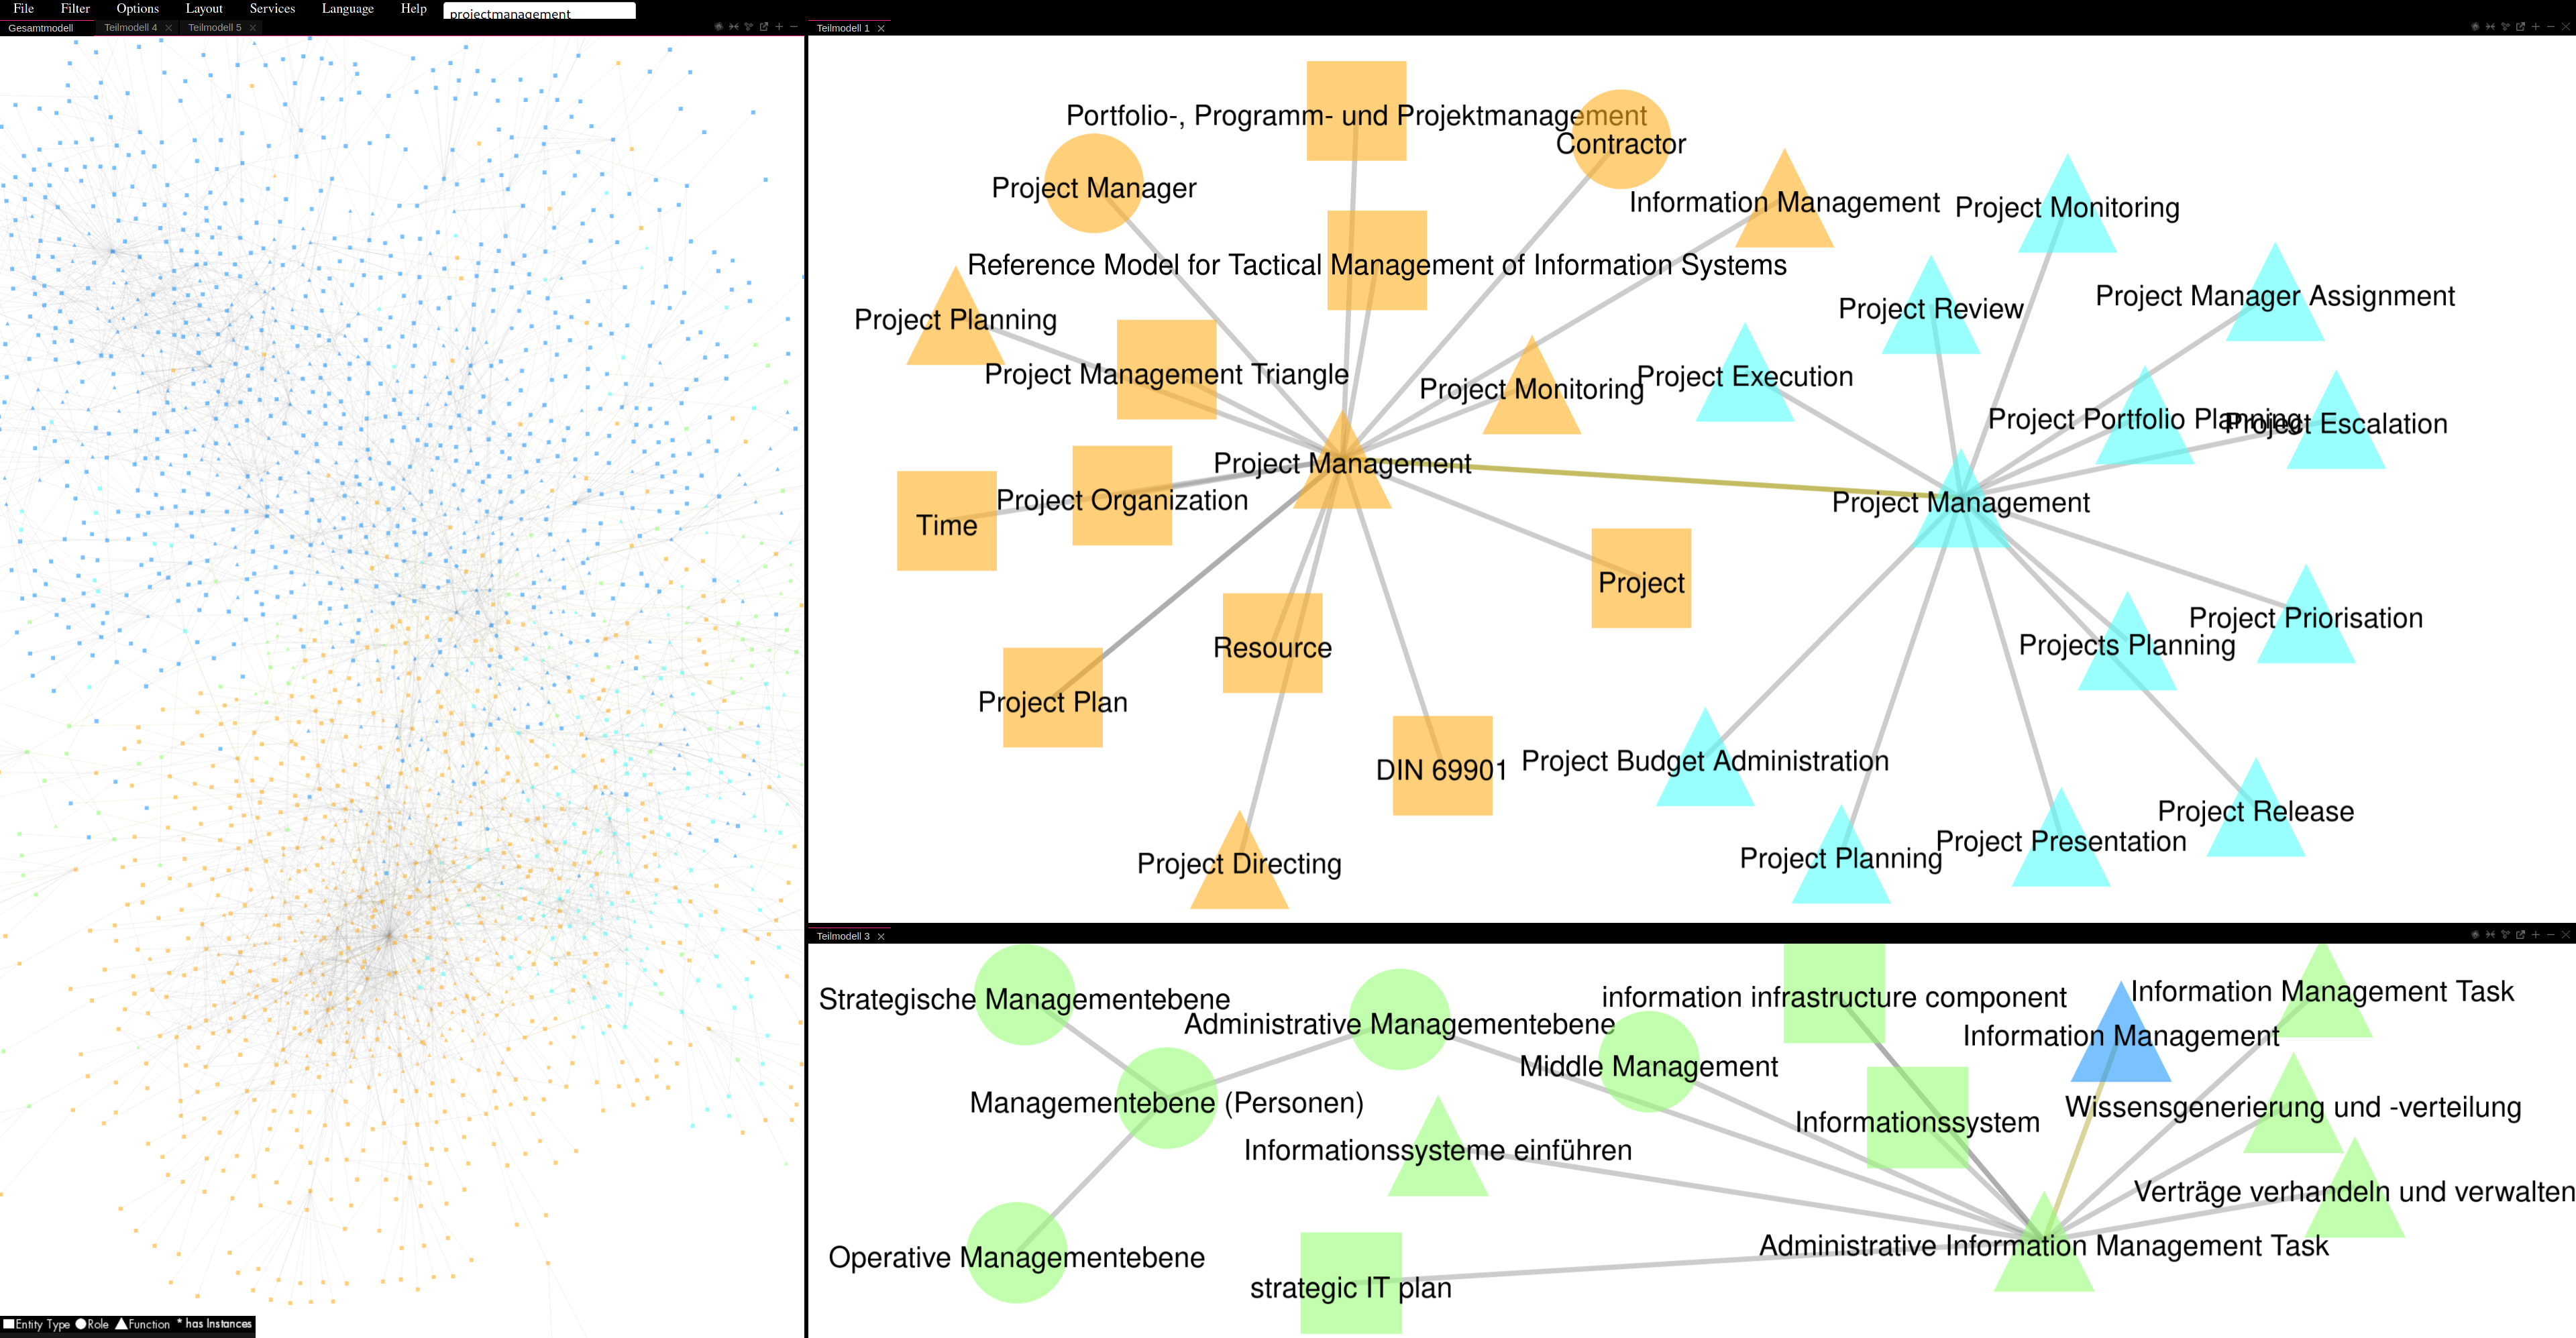
\includegraphics[width=0.5\columnwidth]{img/tabs.png}
%    \caption{A session containing the default view and freely partitioned subgraphs containers.}
%	\label{fig:tabs}
%\end{figure}
%\vspace{-3pt}

%For this subgraphs of the ontology have to be extracted and organized.
%A feature of SNIK Graph, tabs, allows multi-instance usage.
%One major issue in working with SNIK Graph was the missing ability of organizing teaching scenarios.
To organize teaching scenarios, independent SNIK Graph instances are loaded into containers\footnotemark{} that can be organized around the browser window.
\footnotetext{Implemented using the JavaScript GoldenLayout framework (\url{https://golden-layout.com/}).} 
These containers can either be accessed as tabs or freely partitioned.% see \cref{fig:tabs}.
The content and of the all containers can be saved and loaded as a session to continue developing a teaching scenario at a later point.

%This feature allows better workflows in preparation and presentation of teaching scenarios.
%We use JSON formatted files for export and import.

\paragraph{Compound Layout}
%\begin{figure}[h]
%    \centering
%    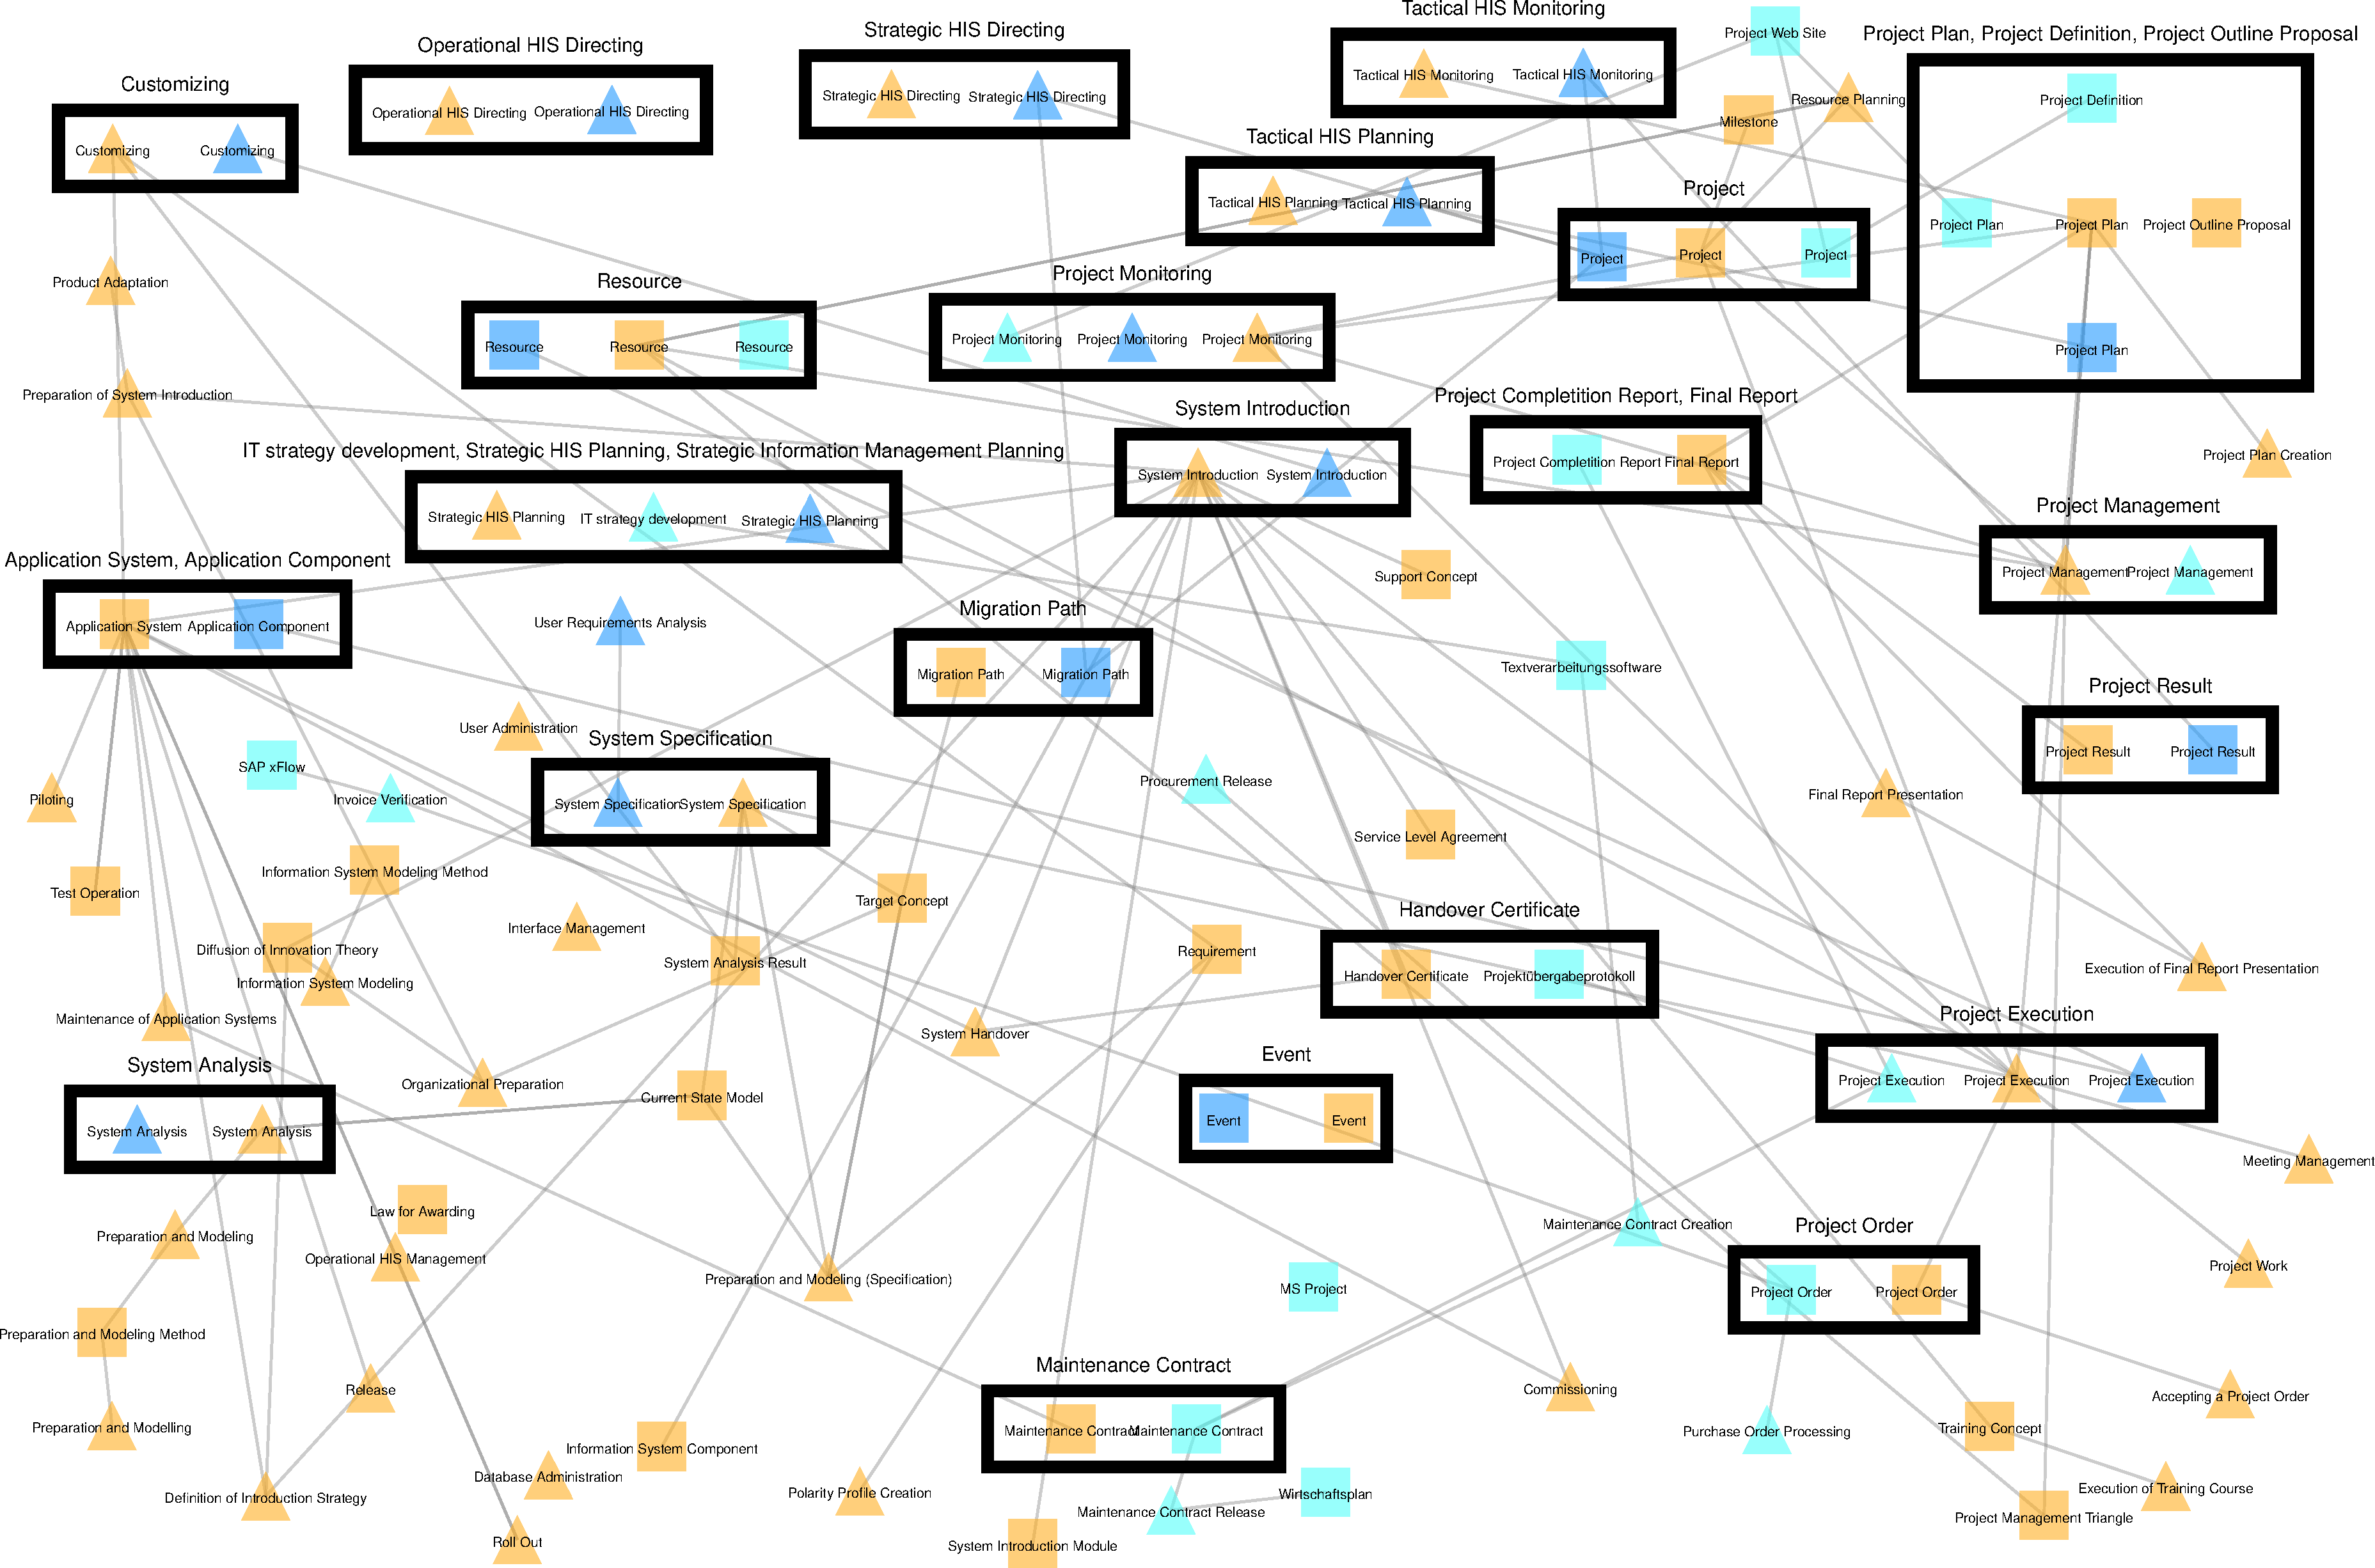
\includegraphics[width=0.5\columnwidth]{img/combine.pdf}
%    \caption{Grouping of equivalent concepts from different sources in SNIK Graph (color coded).}% using the \enquote{combine matches} option.}
%	\label{fig:combine}
%\end{figure}
%\vspace{-3pt}

%\noindent For citations of references, we prefer the use of square brackets and consecutive numbers, e.g. as shown by Author et al. [2], [3, pp. 5–10], as mentioned earlier [1], [3], [9]. The following bibliography provides the basic formats as a reference list with entries for journal articles [1], book chapter [2], as well as a URL [5]. For further guidance please refer to the \href{https://ieeeauthorcenter.ieee.org/wp-content/uploads/IEEE-Reference-Guide.pdf}{IEEE-Reference-Guide}.

Users can group interlinked nodes together and either display them side by side or on top of each other.%, see \cref{fig:combine}.
As SNIK consists of more than 4000 classes, viewing large parts of it at once does not convey much information.%, see \cref{fig:much}.
To alleviate this, SNIK offers multiple exploration methods described in the following.
%\begin{figure}[h!]
%    \centering
%    \includegraphics[width=\linewidth]{much.pdf}
%    \caption{Excerpt of SNIK using the default force directed layout.}\label{fig:much}
%\end{figure}

\paragraph{Role Use}

%\todo{konrad an alle: was mache ich mit der sparql query? rausschmeissen, drin lassen oder umbauen? TP: drinlassen, aber direkt ans Bild hängen.. Sowas wie aus der Query folgt dieses Bild. Ich finde sowas sollte schon rein ins Paper}
%\begin{figure}[h]
%\begin{lstlisting}
%SELECT DISTINCT ?inner ?middle ?outer ?outerx {
% <role> (rdfs:subClassOf|skos:closeMatch|^skos:closeMatch)* ?inner.
% ?inner meta:subTopClass meta:Role.
% OPTIONAL {
%  ?inner ?p ?middle.
%  ?middle meta:subTopClass meta:Function.
%  OPTIONAL {
%   ?middle ?q ?outer.
%   ?outer meta:subTopClass meta:EntityType.
%   OPTIONAL {?outer (skos:closeMatch|^skos:closeMatch|^rdfs:subClassOf)+ ?outerx.}
%}}}
%\end{lstlisting}
%\caption{SPARQL query to generate the \emph{class use} visualization.}
%\label{lst:roleuse}
%\end{figure}
%\vspace{-3pt}

A frequent question is, what a given role does and which information is needed for those functions represented by the entity types connected to those functions.
This question is visually answered by the \enquote{role use} feature, which arranges roles, functions and entity types in concentric circles.%, see \Cref{fig:classuse}:

\begin{enumerate}%[align=left, labelwidth=1ex]
\item The first ring consists of the given role and all roles that are connected by a path of \aurl{rdfs}{subClassOf} and \aurl{skos}{closeMatch} edges.
\item The function ring consists of all functions adjacent to roles in the inner ring.
\item The third ring consists of all entity types adjacent to functions in the middle ring.
\item The final ring consists of all entity types that are connected to entity types from the third ring by a path of \aurl{skos}{closeMatch} and reverse \aurl{rdfs}{subClassOf} edges.
\end{enumerate}

\iffalse
\begin{figure}[h!]
    \centering
    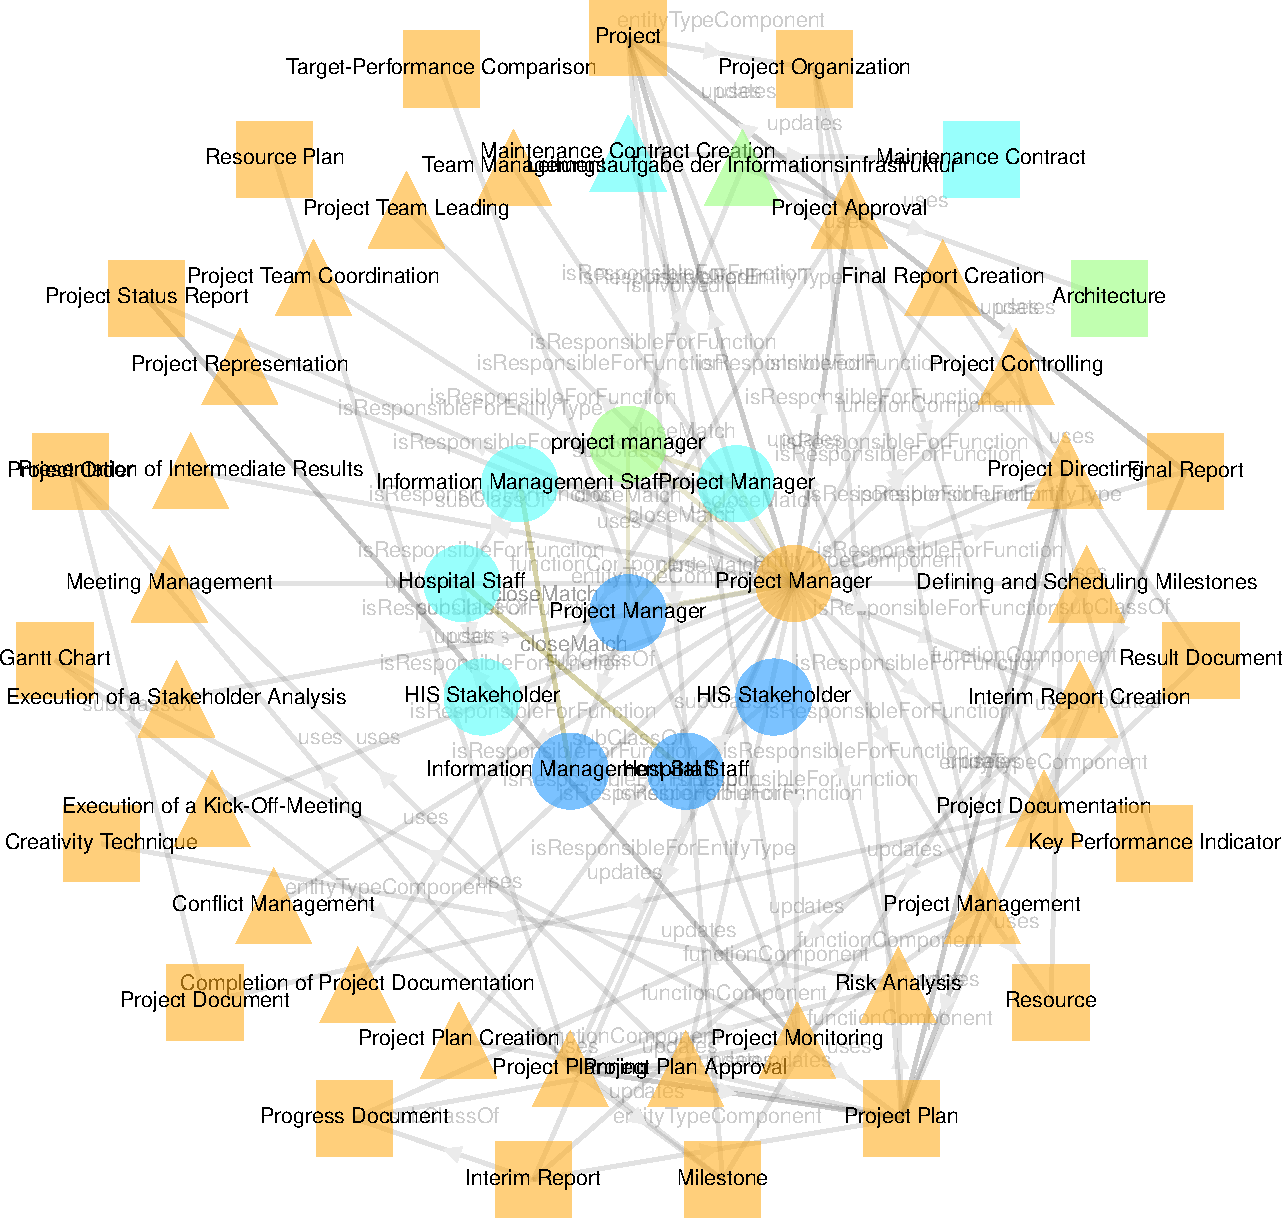
\includegraphics[width=0.5\columnwidth]{img/class-use-project-manager.pdf}
    \caption{\emph{Role Use} of \aurl{bb}{ProjectManager}. Outermost layer ommitted due to space limitiations.}\label{fig:classuse}
\end{figure}
\fi

In SNIK Graph, this operation is called \emph{class use} and allows users to also put a function or entity type in the center.

%\section{Approach}
%Due to its large size, visualizing all of SNIK at once  overplotting.
%At the core of SNIK Graph is incremental exploration, which starts at one or more nodes and gradually expands them to related ones.

\paragraph{Search}
\iffalse
\begin{figure}[h!]
    \centering
    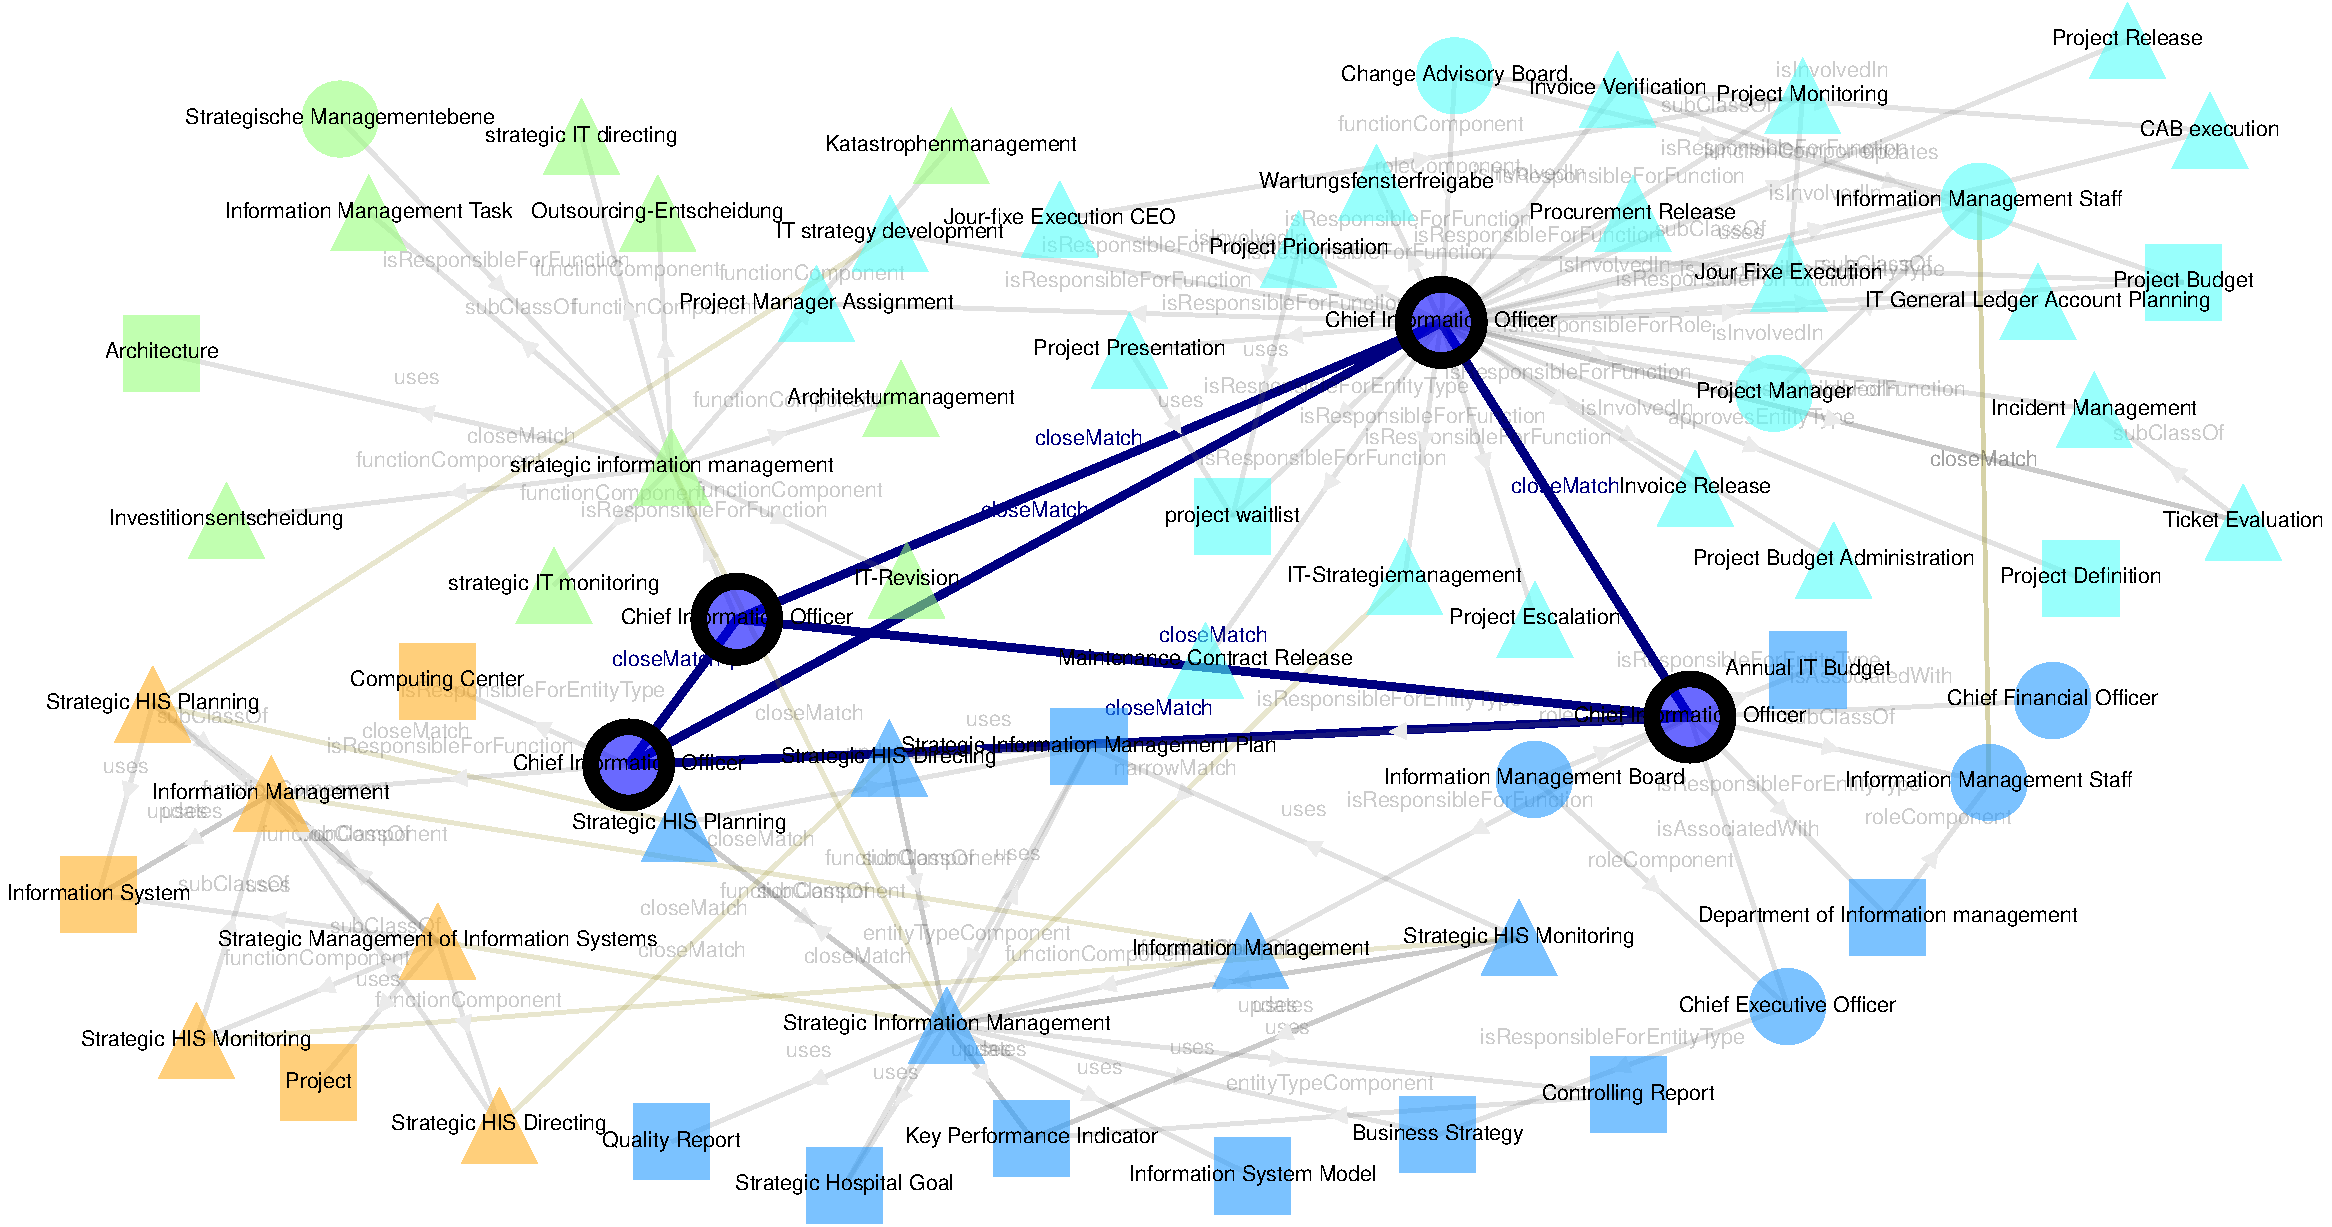
\includegraphics[width=0.5\columnwidth]{img/search.pdf}
    \caption{Visual search results for \enquote{Chief Information Officer} in a part of SNIK.}\label{fig:search}
\end{figure}
\fi
Due to the large amount of resources, exploration often begins with a search.
The search index is populated from the target SPARQL endpoint and is implemented using the Fuse.js library that is based on the Baeza-Yates--Gonnet algorithm~\cite{textsearching}.
Fuse.js\footnotemark{} is a light-weight, purely client side JavaScript library and presents an alternative to backend-driven indexes like Lucene.%
\footnotetext{\url{https://fusejs.io/}, \url{https://github.com/krisk/Fuse}}
This enables fast fuzzy search on any dataset loaded via SPARQL endpoint but requires waiting for index initialization on the first search of each user session.
Search results presented to the user are color coded in three categories: visible (green), invisible (yellow)%
\footnote{The resource is either \emph{filtered} or \emph{hidden}.}% \cref{sec:visibility}
 and not loaded (red)%
\footnote{The resource is included in the search index built from the SPARQL endpoint but either deleted in the graph or not loaded in the first place, such as due to configuration.}.
Each search entry of a class contains the label values of \aurl{rdfs}{label} (long form) and \aurl{skos}{altLabel} (short and alternative forms) with a weight of 0.7.
Textbook definitions are included with a weight of 0.3.
Labels of resources connected via \aurl{skos}{closeMatch} interlinks in either direction are included as well, because those resources are defined as semantically close, so we assume their labels are synonyms.
Fuzzy matching is enabled with a threshold of \num{0.25}.
The resource \aurl{bb}{ChiefInformationOfficer} can thus be found by entering either \enquote{CIO} (alternative label), \enquote{vice president} (part of the definition) or \enquote{Leiter des Rechenzentrums} (German alternative label of \aurl{ob}{ChiefInformationOfficer}).
%Search results are then selected in the graph, see~\cref{fig:search}, which allows further exploration by chaining the path and neighbourhood operations described in following.
Search results are then selected in the graph, which allows further exploration by chaining the path and neighbourhood operations described in following.

\paragraph{Shortest Paths}
\begin{figure}[h!]
    \centering
    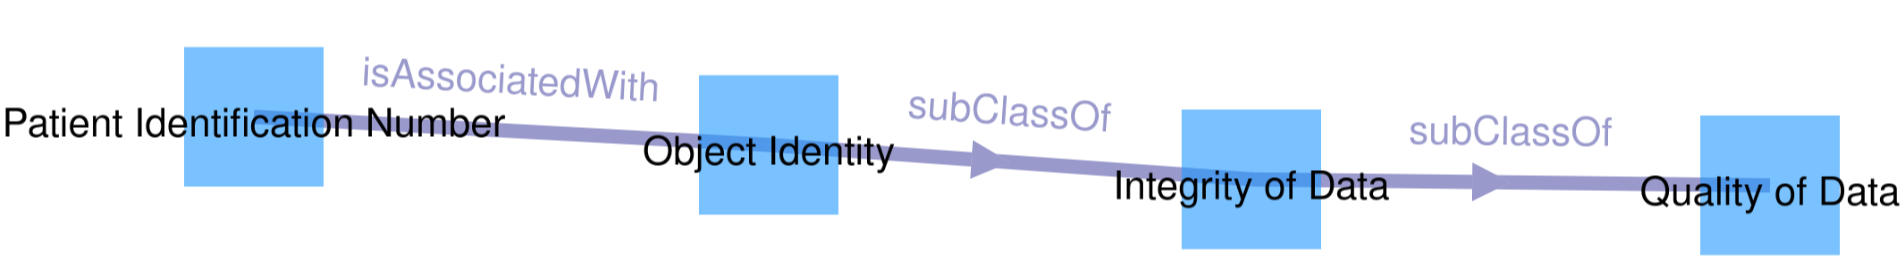
\includegraphics[width=\columnwidth]{img/path.png}
    \caption{The shortest non-trivial path between \aurl{bb}{PatientIdentificationNumber} and \aurl{bb}{QualityOfData} in SNIK Graph.}
	\label{fig:path}
\end{figure}
\vspace{-3pt}
The shortest path is the most basic method of visualizing the relationship between two resources, see \cref{fig:path}.
We treat SNIK as an undirected graph for the calculation because the direction is often arbitrary.
Roles can be nested using \aurl{meta}{roleComponent} (\emph{has part}), which could have just as well been modelled as a \emph{part of} relation with reversed subject and object.
Another reason is that a set of resources that forms a graph connected by some symmetric property implies a complete subgraph, which negatively effects speed, memory and visibility of SNIK Graph.
For this reason, \aurl{skos}{closeMatch} and other symmetrical properties are often only sparsely modelled, and the other triples are implied.
As SPARQL endpoints, such as Virtuoso SPARQL employed by SNIK, do not perform reasoning to infer such implied triples such as those generated by symmetric properties, this would prevent the shortest path from including resources where only the opposite direction is explicitly modelled.%
We also do not explicitly store triples inferred by transitive properties such as \aurl{rdfs}{subClassOf}, which prevents paths involving such properties from being squashed, such as the path between \emph{Project Manager} and \emph{HIS Stakeholder} in \cref{fig:hierarchy}.


%We ignore the direction of edges because, that is, which resource is the subject and the object 
The largest problem of shortest paths is however, that they are not necessarily informative to the user. 
For example, any two roles, such as \aurl{bb}{ChiefInformationOfficer} and \aurl{bb}{ChiefExecutiveOfficer}, are connected by a path of length 2 as they are all subclasses of \aurl{meta}{Role}, which the user already knows given the triangular shapes representing roles in SNIK Graph.
To exclude such trivial paths,  the meta model is not shown by default.
Furthermore, filtering, such as by knowledge source or type of relation or resource, allows further tuning of the resources that are shown and eliglible for paths.
%Further research into informative paths has been done in two bachelor theses~\cite{}.
An general approach to solve the problem of informative shortest paths is \emph{weighted shortest paths for RDF graphs (WiSP)}~\cite{wisp}.
Future work includes adopting this approach to SNIK Graph and evaluating it with its users.
Another approach is to show all short paths under a given length and let the user remove unwanted ones manually, as employed by \emph{Relfinder}~\cite{relfinder}.

\paragraph{Neighbourhood Operations}
Exploration using neighbours, that is the successive uncovering of nodes adjacent to a starting node given by a user, is a common feature of tools such as LodLive~\cite{lodlive} and VizLOD~\cite{vizlod}.%
\paragraph{Star}
The directed and undirected star operations show nodes connected to selected nodes via all paths that contain at most one property other than \aurl{skos}{closeMatch}.
The \emph{circle star} also rearranges the nodes using the force-directed layout locally on the currently visible subgraph.
%\Cref{fig:star} shows a mind map of strategic information management, created by an undirected star, which can be used by a teacher to prepare a lecture about the topic.
\iffalse
\begin{figure}[h!]
    \centering
    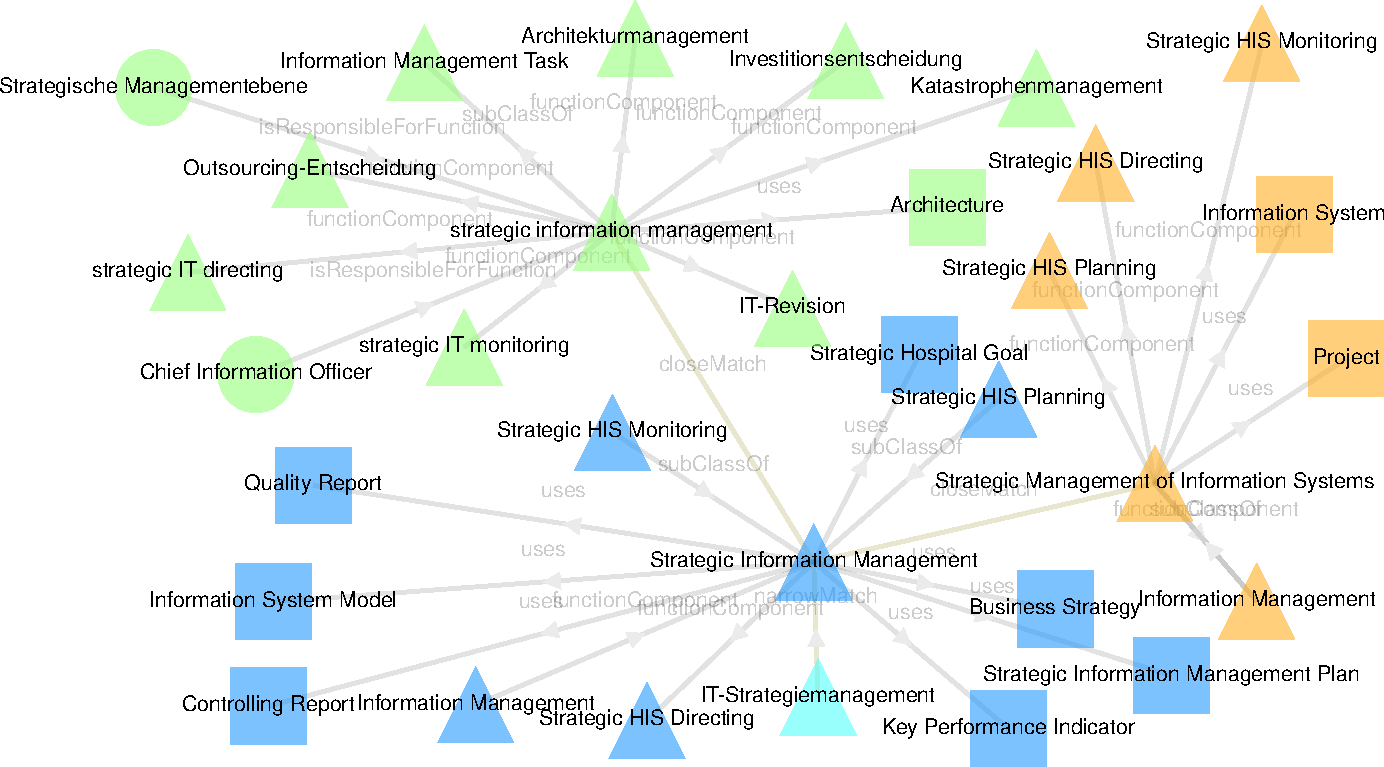
\includegraphics[width=\columnwidth]{img/strategic-im.pdf}
    \caption{Undirected \emph{Star} of \aurl{bb}{StrategicInformationManagement}.}
	\label{fig:star}
\end{figure}
\vspace{-3pt}
\fi

%\todo{Konrad: Nimm den Star um "ob/ProjectManagement".} % ist inkludiert in \cref{fig:tabs}, refer?
The concept \emph{project management} both exists in a textbook~\cite{ob} and in the knowledge about information management in a German university hospital.
Grouping both concepts with the help of the star function the user detects that the terms have a different meaning according to their neighboorhood terms.
Whereas the text book deals with the management of single projects, in the CIO's world \enquote{project management} means managing multiple projects, as shown in the lower right container in \cref{fig:tabs}.
As all neighbourhood and path operations automatically select all resulting nodes, repeated application of a star without clearing the selection results in an incremental uncovering of the whole connected graph around the starting node.

%\subsection{Mixed Operations}
\paragraph{Spiderworm}
A \emph{spiderworm} is a path from node \emph{A} to node \emph{B} combined with a \emph{star} of \emph{B}.
%\Cref{fig:spiderworm} shows how we use a spiderworm to teach a student how the new concept \enquote{quality of data} is connected the the already introduced concept \enquote{patient identification number.}

\iffalse
\begin{figure}[h!]
    \centering
    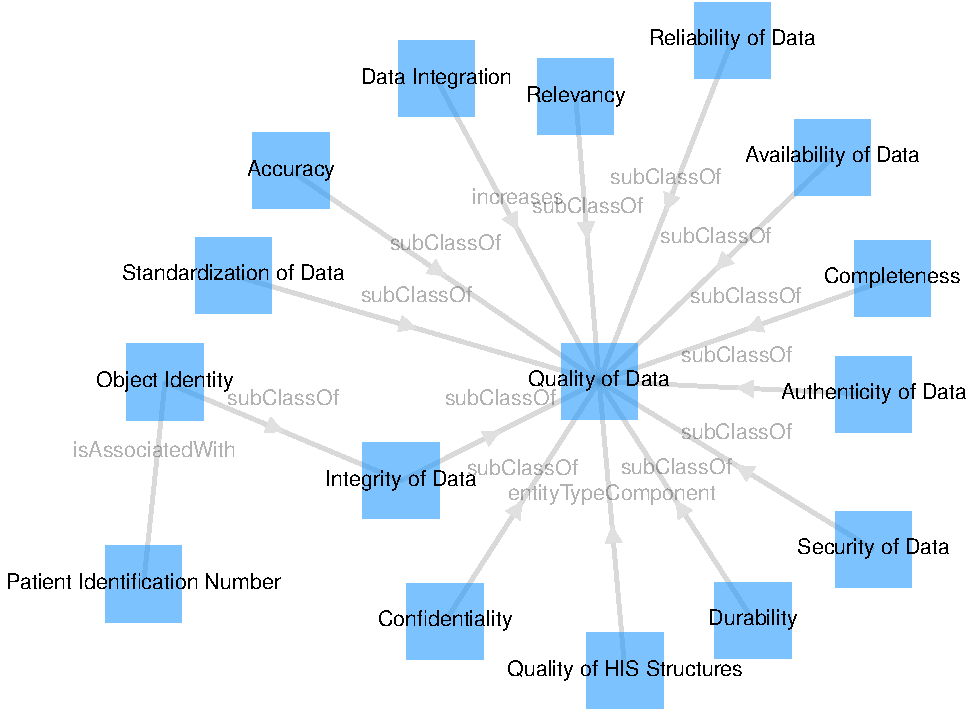
\includegraphics[width=\columnwidth]{img/spiderworm.pdf}
    \caption{\emph{Spiderworm} from \aurl{bb}{PatientIdentificationNumber} to \aurl{bb}{QualityOfData}~\cite{snikgraphposter}.}
	\label{fig:spiderworm}
\end{figure}
\vspace{-3pt}
\fi

\iffalse
Due to the limitations of JavaScript, such as a single thread, and the used library library Cytoscape.js which is the base of the graph visualization, there are performance problems on large graphs.
Right now we have 2641 nodes and 4904 edges and the performance is ok in Chrome but not amazing.
With 10000 nodes it would probably be too slow on most machines.

\todo{reference franziskas poster in both figures}
\todo{get a higher quality version of overview graphic}
\todo{reference \citet{visualizationoflargeontologies}}

\begin{figure}
\caption{SNIK Graph Overview. Source: \protect\citet{snikgraphposter}.}
\label{fig:snik-graph-overview}
\includegraphics[width=\columnwidth]{img/snik-graph.png}
\end{figure}

\begin{figure}
\caption{A teacher prepares a lecture on strategic HIS directing using the \enquote{Circle Star} function of SNIK Graph. Source: \protect\citet{snikgraph}.}
\label{fig:snik-graph-circle-star}
\includegraphics[width=\columnwidth]{img/snik-graph-circle-star.png}
\end{figure}

\begin{figure}
\caption{Students learn new concepts about HIS quality by linking them to concepts already learned.
A teacher asks a student to find out how the new concept \enquote{Quality of Data} is linked to the \enquote{Patient Identification Number}.
The student connects the two concepts by using the “spiderworm“ visualization and learns that a patient identification number is associated with object identity.
Object identity is a subclass of integrity of data.
Besides integrity of data, there are also 13 other criteria for quality of data.}
\label{fig:snik-graph-spiderworm}
\includegraphics[width=\columnwidth]{img/snik-graph-spiderworm.png}
\end{figure}
\todo{FJ: In diesem Abschnitt fehlt die Diskussion, wie es durch die verschiedenen Zielgruppen bei Use Cases genutzt werden kann.}
SNIK Graph is a web application\footnote{\url{http://www.snik.eu/graph}} that transforms the classes and triples of SNIK to nodes and edges of a graph.
The graph is visualized using the Cytoscape.js~\citep{cytoscape} library with the force-directed Euler layout, see~\cref{fig:snik-graph-overview}.
With several thousand classes, specific parts of SNIK can be hard to discern.
Thus, there are several options to view subgraphs of SNIK, for example to show only a specific chapter of a book to prepare a lecture about a specific topic.
Users can also search for and restrict the view to a single class and then show the neighbourhood of that class (see \cref{fig:snik-graph-circle-star}) and subsequently the neighbourhood of selected neighbours of the previous step.
SNIK Graph can also calculate the shortest path to between classes.
We also tried to automatically find the most interesting path but this was not successfull as it is subjective and the depends on the goal of the user.
Path and neighourhood operations are joined in the \enquote{spider worm} (see \cref{fig:snik-graph-spiderworm}), which consists of the shortest path between a start node and an end node together with the end node’s neighbourhood, illustrate the context of a concept.
\fi
\subsection{Quiz}

\begin{table}[t]
\caption{Initial Quiz question templates.}
\label{tab:templates}
\centering
\begin{tabulary}{\columnwidth}{lL}
\toprule
\textbf{Template}	&\textbf{Description}\\
\midrule
Definition		&Ask for the class that fits the given textbook definition.\\
Example			&What is defined as \enquote{Examination of in and out patients in radiological department}?\\
Distractors		&Labels of other classes (that have a path of length 2 or less to the correct class.)\\
\midrule
Subject			&Ask for the class that is related via a given relation to a given object.\\
Example			&Who is \emph{involved in} a \emph{healthcare network}?\\
Distractors		&Labels of other classes (of the same type) that \emph{are not} related via the same relation to the same object.\\
\bottomrule
\end{tabulary}
\end{table}

Clover Quiz~\citep{cloverquiz} shows that ontologies can be used to automatically generate multiple-choice questions over DBpedia~\citep{dbpedia}.
We apply this approach to SNIK and generate 1231 English questions using the templates described in \cref{tab:templates}.
It was used by students from the Universities of Amsterdam, Heidelberg and Leipzig during the international Frank van Swieten lectures in 2019.
To provide difficult wrong answers, the so called \emph{distractors}, we use direct neighbours of the classes that represent the correct answers.
Due to the limited nesting capabilties of SPARQL, which does not support loops but only subqueries that cannot access variables declared outside their scope, querying for distinct sets of 4 neighbours, where exactly one was connected over a certain property to a certain object, was not possible with our Virtuoso SPARQL endpoint initially.
We circumvented the timeout by calculating the neighbour-relation as a first step and uploading it to the endpoint.
%
%SNIK Quiz is freely available as an open source web application.
Because SNIK only contains the knowledge that the source textbooks describe, it does not contain the complete domain of Hospital Information Management.
As such, negative questions are problematic, as the given relationship could hold in the real world but not be described in the textbook source of the class.
The same problem concerns the distractors of positive questions.
So this problem cannot be avoided.
However, this is one of the reasons that we do not ask count questions like \enquote{How many functions is the CIO responsible for?}, which do not help much for learning anyways. % improve writing
Relationships could also hold implicitly through the subclass hierarchy.
For example, \aurl{bb}{ChiefInformationOfficer} is a subclass of \aurl{bb}{InformationManagementStaff}, which is responsible for \aurl{bb}{OperationalInformationManagement}.
It is unclear, whether the CIO is also responsible for operational information management.
An ongoing bachelor's thesis~\citep{snikquiz} is investigating different strategies of generating complex questions, answers and distrators.





%The technical environment of SNIK is characterized in previous work [11].
\iffalse
\section{Discussion}
SNIK is based on the meta model from Figure \todo{reference}.
Thus, SNIK can be considered as an archetype for ontologies describing for a given domain (here \enquote{HIS management}), what functions a certain role has to carry out and what information a person of this role needs and what information she/he provides while carrying out the functions.
This may be used for domains like the medical department of a hospital as well.\todo{FJ: Ich glaube, das müsste man ausführlicher erklären, das würde ich eher ans Ende der Diskussion nehmen.}
This would be valuable knowledge, for instance as basis for systems analysis projects [1].
Different user groups can use the interfaces of SNIK that are most suitable to them.
For example, the IT management of a hospital can use SNIK as a vocabulary to integrate data from different formats that result from application components from different vendors.
Using the SPARQL query language, experts can also integrate applications with the SNIK ontology.
 Experts can also use the SPARQL query editor to answer specific questions, see Table 2.
Students and teachers, on the other hand, benefit more from SNIK Graph, which intuitively presents knowledge without the need for technical skills.

Figure 4– A \enquote{Spider Worm} between the classes \enquote{Change Management} and \enquote{HIS Quality} in the SNIK Graph visualization web application.
The content of SNIK is taken from textbooks which are protected by property rights of publishing houses or taken from an interview with a CIO holding property rights as well.
Making the SNIK ontology openly available may therefore conflict with these property rights.
In case of SNIK, we appreciate the approvals of the publishing houses Springer, de Gruyter and Schattauer and of the CIO.
In general, missing approvals may prevent the creation of such open ontologies and thus the provision of textbook content as open knowledge.
The approvals for SNIK were possible because for each class and relation being part of SNIK there is a clear indication of its source (see code \enquote{bb} and chapter information in Table 1).
In future work we will use these indications for establishing hyperlinks into the sources such that users of SNIK may use SNIK as a smart index for retrieving more detailed knowledge and supporting illustrations from the original textbooks – if digitally available.
We are convinced that this way an ontology like SNIK is not a competitor of textbooks but a smart guide for using a textbook.
Thus, it might be attractive for publishing houses.
\fi
\todo{verweis auf existierende papers}
\todo{benutzung durch braunschweig}
\todo{benutzung durch amsterdam}

\section{Discussion}
We showed that knowledge on the management of information systems in medicine and health care is made publicly available using open standards over several interfaces with different compromises between expressivity and accessibility.
It can be combined with other knowledge in biomedical and health informatics and in other disciplines.

%\section{Future Work}
\section{Conclusions}
In the future, we plan to extend the text-based interlinks with semantic-similarity-based ontology matching [5] to find more correspondencies between the textbooks.
This will enable users to switch to another textbook when a certain concept is explained there in more detail.
The SNIK toolset, SNIK Graph in particular, is under permanent improvement.
For instance, we are considering alternatives to the shortest path that are the most preferred by different audiences and whether those paths can be (semi-)automatically generated using suitable node or edge weight functions.
We are also investigating candidates for additional subontologies and as interlink targets.
Past efforts of automatic textbook extractions were unsuccessfull but recent advances in natural language processing, such as GPT-3~\citep{gpt3}, motivate further investigation.

%\section{Acknowledgments}
%This work is supported by the DFG (German Research Foundation) under the Projects SNIK, grant no. 1605/7-1 and 1387/8-1, as well as HITO, grant no. WI 1605/11-1 and I3726-N31.
%We thank the publishers ... and ... for granting us permission to publish the subontologies based on the textbooks \citet{bb,ob,he} under an open license.
%\nocite{*} 
\todo{FJ: Hmmm, ziemlich selbstreferenziell. Brauchen wir da wirklich so viele Publikationen von uns? Welche anderen könnte man noch einbringen? Ich schaue auch mal, was mir so über den Weg läuft.}
%\bibliographystyle{ios1}
\bibliographystyle{vancouver}
\bibliography{paper,snik,relatedwork}
%\section{Notes to Reviewers}
%This paper includes and extends text and figures from:
%\citet{snikgraph}
\end{document}
